% $Header: /cvsroot/latex-beamer/latex-beamer/solutions/conference-talks/conference-ornate-20min.en.tex,v 1.6 2004/10/07 20:53:08 tantau Exp $

\documentclass[11pt]{beamer}

% This file is a solution template for:

% - Talk at a conference/colloquium.
% - Talk length is about 20min.
% - Style is ornate.

% Copyright 2004 by Till Tantau <tantau@users.sourceforge.net>.
%
% In principle, this file can be redistributed and/or modified under
% the terms of the GNU Public License, version 2.
%
% However, this file is supposed to be a template to be modified
% for your own needs. For this reason, if you use this file as a
% template and not specifically distribute it as part of a another
% package/program, I grant the extra permission to freely copy and
% modify this file as you see fit and even to delete this copyright
% notice. 

\mode<presentation>
{
  % Turn off shadowing, large frame titles, and sans-serif fonts
  % (ALL OF WHICH PISS ME OFF - RBN).
  \usetheme{default}
  \usefonttheme{serif}
  \usecolortheme[RGB={0,0,0}]{structure}
  \setbeamercovered{transparent}
  \setbeamerfont{frametitle}{size=\normalsize,series=\bfseries}
}

\usepackage{graphics}

\usepackage[english]{babel}
% or whatever

%\usepackage[latin1]{inputenc}
% or whatever

\usepackage{times}
\usepackage[T1]{fontenc}
% Or whatever. Note that the encoding and the font should match. If T1
% does not look nice, try deleting the line with the fontenc.

% Add a frame indication to the navigation symbols
\setbeamertemplate{navigation symbols}{}
\setbeamertemplate{footline}{
\vskip1mm \ 
{\it \insertshorttitle}
\hfill
Frame \insertframenumber\ of \inserttotalframenumber\ 
\insertslidenavigationsymbol
\insertframenavigationsymbol
\insertsubsectionnavigationsymbol
\insertsectionnavigationsymbol
\insertdocnavigationsymbol
\insertbackfindforwardnavigationsymbol
\  \vskip1mm
}

\setbeamertemplate{bibliography item}[text]{}

\title[Population unattributable fractions and other scenario comparisons] % (optional, use only with long paper titles)
{\textbf{Population unattributable fractions and other scenario comparisons}}

\subtitle
{\scriptsize With examples from the Avon Longitudinal Study of Parents and Children (ALSPAC) cohort study at Bristol University, UK
\\ \href{http://www.bristol.ac.uk/alspac/}{\textsl{http://www.bristol.ac.uk/alspac/}}
}

\author[Author, Another] % (optional, use only with lots of authors)
% {F.~Author\inst{1} \and S.~Another\inst{2}}
{
Roger B. Newson
\\ \href{mailto:r.newson@imperial.ac.uk}{r.newson@imperial.ac.uk}
\\ \href{http://www.imperial.ac.uk/nhli/r.newson/}{\textsl{http://www.imperial.ac.uk/nhli/r.newson/}}
}
% - Give the names in the same order as the appear in the paper.
% - Use the \inst{?} command only if the authors have different
%   affiliation.

%\institute[Universities of Somewhere and Elsewhere] % (optional, but mostly needed)
\institute[National Heart and Lung Institute, Imperial College London]
{
National Heart and Lung Institute\\
Imperial College London
}
\date[Asthma Club 2010] % (optional, should be abbreviation of conference name)
{
Asthma Club, 11~November, 2010
}

\subject{Confounder adjustment}
% This is only inserted into the PDF information catalog. Can be left
% out. 


% If you have a file called "university-logo-filename.xxx", where xxx
% is a graphic format that can be processed by latex or pdflatex,
% resp., then you can add a logo as follows:

% \pgfdeclareimage[height=0.5cm]{university-logo}{university-logo-filename}
% \logo{\pgfuseimage{university-logo}}

\begin{document}

\section{Title}

\begin{frame}
  \titlepage
\end{frame}

\section{Introduction}

%\begin{frame}
%  \frametitle{Outline}
%  \tableofcontents[pausesections]
%  % You might wish to add the option [pausesections]
%\end{frame}

\begin{frame}
\frametitle{Why scenario comparisons?}

\begin{itemize}

\item<2-> Public health scientists make their living mostly by proposing (or fantasizing) \textbf{interventions}.

\item<3-> Such interventions might be helping people to quit smoking, offering informative DNA tests,
or genetic engineering of eggs and sperms.

\item<4-> A skeptical public will ask what good these proposed interventions will do,
especially if they are expensive.

\item<5-> \textit{So} public health scientists need to be able to give an answer.

\item<6-> These answers are comparisons between \textbf{scenarios},
defined as fantasy worlds in which different interventions are made (or not made).

\item<7-> Any two fantasy scenarios compared will be different in some ways, but the same in others.

\end{itemize}

\end{frame}

\begin{frame}
\frametitle{What are scenario comparison statistics?}

\begin{itemize}

\item<2-> In statistics, \textbf{scenarios} can be defined as alternative versions of the same dataset.

\item<3-> \textit{For instance}, we might have a dataset with 1 observation per patient,
and data on age, smoking and lung disease.

\item<4-> And we might compute an alternative version of the same dataset, with the same age distribution,
but all patients lifelong non--smokers.

\item<5-> Lung disease outcome distributions in these two versions can be \textbf{compared} using a \textbf{statistic},
such as a mean difference, a mean ratio, a ratio between means,
a median difference, or a difference between medians.

\item<6-> And all of these comparisons can be presented with confidence limits and $P$--values.

\item<7-> We can therefore estimate the consequences of a proposed intervention,
\textit{assuming} that an association between smoking and lung disease is \textbf{causal},
at least within each age group.

\end{itemize}

\end{frame}

\section{Example from ALSPAC}

\begin{frame}
\frametitle{Example: Asthma and prenatal paracetamol in the ALSPAC cohort}

\begin{itemize}

\item<2-> The Avon Longitudinal Study of Parents and Children (ALSPAC) is a birth cohort study,
based at Bristol University, with 14060 subjects, born in the early 1990s.

\item<3-> The following example revisits a subset of the dataset discussed
in Shaheen \textit{et al.}, 2010\cite{shaheen2010}.

\item<4-> The \textbf{outcome} of primary interest, in this example,
is doctor--diagnosed asthma at any time
from 0--91 months of age.

\item<5-> The \textbf{exposure} is self--reported maternal paracetamol consumption
during weeks 20--32 of pregnancy
(``Never'', ``Sometimes'' or ``Most days/daily'').

\item<6-> The proposed \textbf{intervention} is presumably the replacement of paracetamol
with some unspecified other drug
as the analgesic of choice for pregnant mothers.

\item<7-> The \textbf{candidate confounder list} was $\ldots$

\end{itemize}

\end{frame}

\begin{frame}
\frametitle{Candidate confounders}

\begin{itemize}

\item<2-> $\ldots$ gender, maternal age group, prenatal tobacco exposure,
maternal education, maternal housing tenure,
parity, maternal anxiety group,
maternal ethnic origin, multiple pregnancy,
birth weight, gestational age at birth, head circumference at birth,
maternal antibiotic use in pregnancy,
alcohol exposure (0--8 weeks gestation, 0--18 weeks gestation, 18--32 weeks gestation, last 2 months gestation),
maternal pre--pregnancy disease history (asthma, eczema, rhinoconjunctivitis, migraine),
maternal infection history during pregnancy (colds/flu, urinary, other),
younger siblings at 7 years, pets in first year, breast feeding in first 6 months,
day care in first year, damp in home, 
weekend environmental tobacco exposure in first year,
child's BMI at 7 years.

\item<3-> Most of these are not likely to be ``causally upstream'' from prenatal paracetamol or asthma,
but might indicate aspects of health and/or wealth that might influence both,
and which are probably unaffected by analgesic substitution.

\end{itemize}

\end{frame}

\begin{frame}
\frametitle{Confounder adjustment: Propensity scores}

\begin{itemize}

\item<2-> In the ALSPAC cohort, the mothers of 12127 children gave information on paracetamol use
during weeks 20--32 of pregnancy.

\item<3-> We defined a paracetamol--propensity score for each of these children,
based on the listed confounders,
using an ordinal logistic regression model,
as proposed by Lu \textit{et al.}, 2001\cite{lu2001}.

\item<4-> These 12127 children were grouped into 32 nearly--equal propensity groups,
based on the propensity score.

\item<5-> All of these propensity groups were represented
in the subset of 7704 of these children
with data on doctor--diagnosed asthma at ages up to 91 months.

\end{itemize}

\end{frame}

\begin{frame}
\frametitle{Histograms of paracetamol propensity group by paracetamol exposure}

\begin{columns}[t]
\begin{column}{48mm}
\begin{itemize}
\item<2-> Paracetamol propensity seems to predict paracetamol exposure,
but not \textit{too} well.
\item<3-> All 32 propensity groups are represented in the unexposed group.
\item<4-> \textit{Therefore}, we should be able to contrast asthma risk
between the real world and a fantasy scenario,
with the same propensity distribution but no exposure.
\end{itemize}
\end{column}
\begin{column}[T]{80mm}
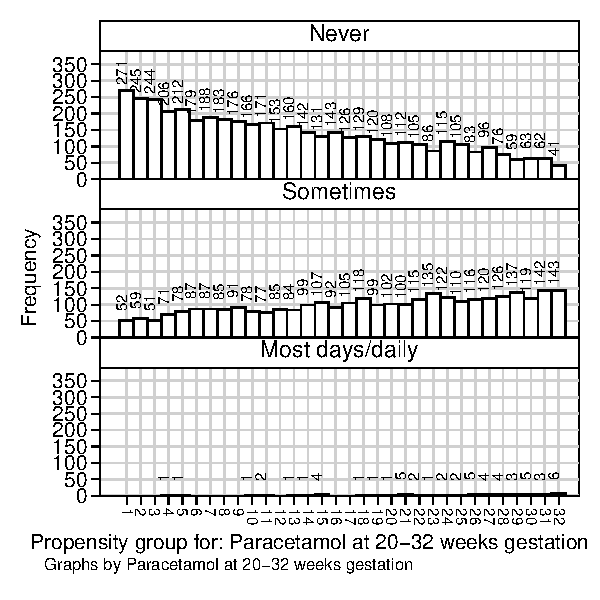
\includegraphics[width=76mm]{figseq1.pdf}
\end{column}
\end{columns}

\end{frame}

\section{Method 1: Population attributable fractions by logistic regression}

\begin{frame}
\frametitle{Method 1: Logistic regression and the population attributable fraction (Greenland and Drescher, 1993\cite{greenland1993})}

\begin{itemize}

\item<2-> We fitted a propensity--adjusted logistic regresssion model,
with a baseline odds of asthma for each propensity group,
and an odds ratio for each non--zero paracetamol exposure level.

\item<3-> This model does not assume that paracetamol effects are ``linear'' per exposure category,
but assumes that they are the same in all paracetamol--propensity groups.

\item<4-> We then used the \texttt{punaf} add--on package,
available in Version~11 of Stata,
to estimate the \textbf{population unattributable fraction (PUF),}
assuming this model.

\item<5-> The PUF is a ratio between asthma risks
in a fantasy scenario, with the same propensity distribution and no exposure,
and asthma risks in the real world.

\item<6-> The PUF, and its confidence limits, are subtracted from 1
to give a confidence interval for the \textbf{population attributable fraction (PAF)},
assuming the same model.

\end{itemize}

\end{frame}

\begin{frame}
\frametitle{Adjusted odds ratios of asthma with respect to paracetamol exposure}

\begin{columns}[t]
\begin{column}{48mm}
\begin{itemize}
\item<2-> Paracetamol exposure is associated with increased asthma,
even allowing for paracetamol propensity.
\item<3-> \textit{However}, we would like to have a summary of overall trend.
\item<4-> And it would be even better if it indicated how much good might be done
by replacing paracetamol with a ``harmless'' analgesic.
\end{itemize}
\end{column}
\begin{column}[T]{80mm}
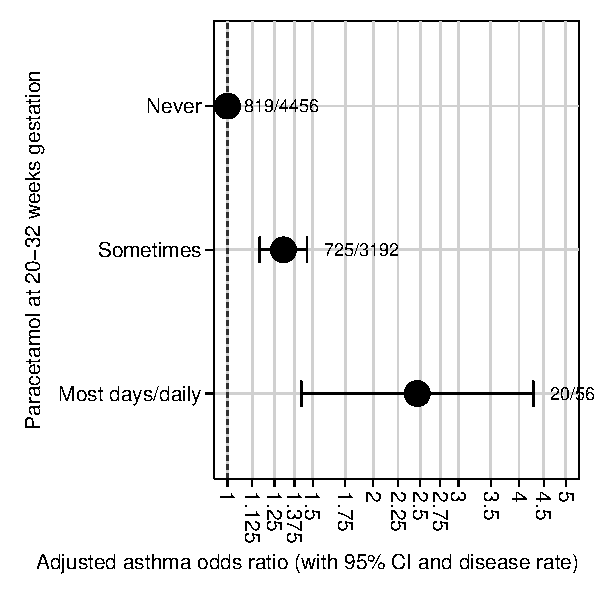
\includegraphics[width=76mm]{figseq2.pdf}
\end{column}
\end{columns}

\end{frame}

\begin{frame}[fragile]
\frametitle{Scenario means and population unattributable and attributable fractions}

After fitting the logistic regression model,
we use \texttt{punaf} to compute the scenario means (asthma risks)
and population unattributable and attributable fractions:

\tiny
\begin{verbatim}
. punaf, atspec(para32g=0) eform post;

Confidence intervals for the scenario means
under Scenario 0 (baseline) and Scenario 1 (specified by atspec() option)
and for the population unattributable faction (PUF)
Total number of observations used: 7704
------------------------------------------------------------------------------
             | Mean/Ratio   Std. Err.      z    P>|z|     [95% Conf. Interval]
-------------+----------------------------------------------------------------
  Scenario_0 |   .2030114    .004558   -71.02   0.000     .1942717    .2121444
  Scenario_1 |   .1889629   .0060648   -51.91   0.000     .1774423    .2012314
         PUF |   .9307992    .020928    -3.19   0.001     .8906717    .9727347
------------------------------------------------------------------------------

95% CI for the population attributable fraction (PAF)
                Estimate     Minimum     Maximum 
         PAF   .06920077   .02726535   .10932832 
\end{verbatim}
\normalsize

``Scenario\_0'' is the real world of our sample.
``Scenario\_1'' is the fantasy sample with the same propensity distribution
and no exposure.
And the PUF is the ``Scenario\_1''/``Scenario\_0'' asthma risk ratio,
which can be subtracted from 1 to derive the PAF.

\end{frame}

\begin{frame}
\frametitle{Method 1: Summary of results}

\begin{itemize}

\item<2-> Under ``Scenario 0'' (the real world),
20.30\% of subjects (95\% CI, 19.43\% to 21.21\%)
had ever had doctor--diagnosed asthma by the age of 91 months.

\item<3-> Under ``Scenario 1'' (the same distribution of ``paracetamol proneness''
but no paracetamol exposure),
the risk might be 18.90\%
(95\% CI, 17.74\% to 20.12\%).

\item<4-> The ratio of the second risk to the first (the PUF)
is .9308 (95\% CI, .8907 to .9727),
indicating that 89 to 97 percent of the risk would remain
if paracetamol exposure was eliminated but confounding factors stayed the same.

\item<5-> \textit{So} the PAF
(the fraction of lifetime asthma risk attributable to prenatal paracetamol exposure)
is 6.92\% of the total risk (95\% CI, 2.73\% to 10.93\%).

\item<6-> Most people would \textit{probably} understand this message more easily than the odds ratios.

\end{itemize}

\end{frame}

\section{Method 2: Population attributable risks by direct standardization}

\begin{frame}
\frametitle{Method 2: Direct standardization and the population attributable risk
(Newson, 2006\cite{newson2006})}

\begin{itemize}

\item<2-> The \textbf{population attributable risk (PAR)} is defined by Gordis (2000)\cite{gordis2000}
as a scenario \textit{difference} between disease risks.

\item<3-> ``Scenario 0'' is the real world of the sample we have,
and ``Scenario 1'' is a fantasy scenario with no exposure to the risk factor.

\item<4-> This concept is easily generalized, using direct standardization,
to the case where Scenarios~0 and 1
are assumed to have the same distribution of one or more categorical confounders.

\item<5-> In this case, the alternative scenarios (versions of the data)
are distinguished by alternative sampling--probability weights.

\item<6-> These sampling--probability weights are 1 for all subjects in Scenario~0.

\item<7-> In Scenario~1, they are 0 for exposed subjects,
and equal, in an unexposed subject, to the ratio of its confounder--group frequency in all subjects
to its confounder--group frequency in unexposed subjects.

\end{itemize}

\end{frame}

\begin{frame}
\frametitle{The population attributable risk as a rank statistic}

\begin{itemize}

\item<2-> Arguably, a difference between proportions is more naturally a rank statistic than a regression statistic,
although it can be either.

\item<3-> It is defined as a special case of Somers'~$D$,
which in general is a difference between probabilities of concordance and discordance.

\item<4-> Sensible Normalizing and variance--stabilizing transforms for a difference between proportions
include the arcsine and the hyperbolic arctangent (also known as Fisher's~$z$).

\item<5-> (This is in contrast to the proportions themselves,
for which a sensible transformation is the log odds.)

\item<6-> The \texttt{scsomersd} add--on package, available in Version~10 of Stata,
estimates a range of scenario--comparison rank statistics, including the PAR,
using scenario--specific sampling--probability weights.

\end{itemize}

\end{frame}

\begin{frame}
\frametitle{Example: Paracetamol exposure and asthma in ALSPAC}

\begin{itemize}

\item<2-> The exposure is late pre--natal paracetamol exposure (at any level).

\item<3-> The outcome is doctor--diagnosed asthma (ever by age 91 months).

\item<4-> The confounder groups are the 32 paracetamol--propensity groups.

\item<5-> The sampling--probability weights in Scenario~1 (elimination of paracetamol exposure)
are equal, for each unexposed subject, to the ratio between the frequencies of its propensity group
in all subjects and in unexposed subjects.

\item<6-> We computed the scenario risks from scenario odds,
using logistic regression with sampling--probability weights,
and the directly--standardized difference between these risks,
using \texttt{scsomersd}.

\end{itemize}

\end{frame}

\begin{frame}[fragile]
\frametitle{Estimation of population attributable risk using \texttt{scsomersd}}

The specification \texttt{pwei=1} specifies sampling--probability weights in Scenario 0.
The option \texttt{sweight(dsweight*(exposed==0))} specifies sampling--probability weights
in Scenario 1.

\tiny
\begin{verbatim}
. scsomersd ddasth91 [pwei=1], sweight(dsweight*(exposed==0)) transf(z) tdist;
Von Mises Somers' D with variable: _scen0
Transformation: Fisher's z
Valid observations: 12160
Number of clusters: 7704
Degrees of freedom: 7703

Symmetric 95% CI for transformed Somers' D
                                (Std. Err. adjusted for 7704 clusters in _obs)
------------------------------------------------------------------------------
             |              Jackknife
      _scen0 |      Coef.   Std. Err.      t    P>|t|     [95% Conf. Interval]
-------------+----------------------------------------------------------------
       _yvar |   .0114349   .0045842     2.49   0.013     .0024486    .0204213
------------------------------------------------------------------------------

Asymmetric 95% CI for untransformed Somers' D
                Somers_D     Minimum     Maximum 
       _yvar   .01143442   .00244855   .02041844 
\end{verbatim}
\normalsize

The output is in alien--looking language.
\textit{However}, the bottom line (giving the PAR)
is the part that we can communicate to pregnant mothers and health professionals.

\end{frame}

\begin{frame}
\frametitle{Method 2: Scenario risks and the population attributable risk}

\begin{tabular}{rrrrrl}
\hline
\textit{Scenario}&\textit{N}&\textit{Risk}&\textit{(95\%}&\textit{CI)}&\textit{P}\\
\hline
Scenario 0&$7704$&$0.2030$&$(0.1942,$&$0.2121)$&$$\\
Scenario 1&$4456$&$0.1916$&$(0.1795,$&$0.2043)$&$$\\
PAR&$7704$&$0.0113$&$(0.0024,$&$0.0200)$&$.013$\\
\hline
\end{tabular}

\bigskip

\begin{itemize}

\item<2-> We see that,
\textit{if} we substituted a ``harmless'' analgesic for paracetamol during pregnancy,
\textit{and} ``paracetamol proneness'' remained the same,
\textit{then} we might save 1\% of children from ever having asthma, at least up to 91 months of age.

\item<3-> This percent (and its confidence limits) will look more exciting
if multiplied by the total population of children in the UK.

\item<4-> Note that the asthma risk under Scenario~1 by Method~2
is slightly different from the asthma risk under Scenario~1 by Method 1,
as we are no longer assuming paracetamol odds ratios to be constant between propensity groups.

\end{itemize}

\end{frame}

\section{Summary and future improvements}

\begin{frame}
\frametitle{Summary: Methods~1 and 2}

\begin{itemize}

\item<2-> Both of these methods produce measures of overall trend
that are easier to understand than odds ratios.

\item<3-> Method~1 estimates scenario risks and population attributable \textit{fractions}
(proportions of \textit{ever--asthmatics} that might have been saved).

\item<4-> This is done using a logistic regression model,
which assumes common paracetamol odds ratios for all sets of confounder values.

\item<5-> Method~2 estimates scenario risks and population attributable \textit{risks}
(proportions of \textit{all children} that might have been saved).

\item<6-> This is done by direct standardization, and does not assume a logistic model,
or any other regression model.

\item<7-> \textit{However}, direct standardization does require that unexposed subjects
are represented in each paracetamol--propensity group.

\end{itemize}

\end{frame}

\begin{frame}
\frametitle{Future improvements}

\begin{itemize}

\item<2-> I plan to extend \texttt{punaf} to estimate population unattributable and attributable fractions for case--control studies.

\item<3-> It would also be good to make all these methods easier for non--technical people to use.

\end{itemize}

\end{frame}

\section{References}

\begin{frame}
\frametitle{References}

\setbeamerfont{text}{size=\small}

{\scriptsize

\begin{thebibliography}{10}

\bibitem{gordis2000}
Gordis L.
\textsl{Epidemiology. 2nd ed.} 2000; Philadelphia, PA: W. B. Saunders.

\bibitem{greenland1993}
Greenland S, Drescher K.
Maximum likelihood estimation of the attributable fraction from logistic models.
\textsl{Biometrics} 1993; \textbf{49(3)}: 865--872.

\bibitem{lu2001}
Lu B, Zanutto E, Hornik R, Rosenbaum PR.
Matching with doses in an observational study of a media campaign against drug abuse.
\textsl{Journal of the American Statistical Association} 2001; \textbf{96}: 1245--1253.

\bibitem{newson2006}
Newson R.
Confidence intervals for rank statistics: Somers'~$D$ and extensions.
\textsl{The Stata Journal} 2006; \textbf{6(3)}: 309--334.

\bibitem{shaheen2010}
Shaheen SO, Newson RB, SM, Rose-Zerilli MJ,Holloway JW, Henderson AJ.
Prenatal and infant acetaminophen exposure, antioxidant gene polymorphisms and childhood asthma.
\textsl{Journal of Allergy and Clinical Immunology} 2010, in press.
doi:~10.1016/j.jaci.2010.08.047.

\end{thebibliography}

}

\bigskip

\end{frame}

\end{document}
